\documentclass[../main.tex]{subfiles}

\begin{document}


\section{Definitions of different types of distributions}
\subsection{The Binomial Distribution}

The probability of a success is denoted by p. \\
The probability of a failure is then 1 - P\\
Such a trial is called a Bernoulli trial with success probability p.\\
The number of successes is then a random variable, which is said to have a binomial distribution.\\
If $X\sim Bin(n,p)$, then the mean and variance of X are given by:
\begin{align*}
    \mu _x &= np\\
    \sigma _x^2 &=np(1-p)
\end{align*}

\subsection{The Poisson Distribution}
The Poisson distribution is as an approximation to the binomial distribution when n is large and p is small.\\
The mass function depends almost entirely on the mean np, and very little on the specific values of n and p. 
We can therefore approximate the binomial mass function with a quantity $\lambda=np$.\\
$\lambda$ is the parameter in the Poisson distribution.\\
If \xsim Poisson($\lambda$), then\\
X is a discrete random variable whose possible values are the non-negative integers.\\
$\lambda$ must be positive constant.\\
The PMF of X is:
\begin{equation*}
    p(x)=P(X=x)=
    \begin{cases}
    e^{-1}\lambda^{x} &, x=0,1,2,...\\
    0 &, \mbox{otherwise}
    \end{cases}
\end{equation*}
The mean and variance are
\begin{align*}
    \mu_X &= \lambda\\
    \sigma_X^2 &= \lambda
\end{align*}
The Poisson PMF is very close to the binomial PMF when n is large p is small and $\lambda = np$.

\subsection{The Normal Distribution}
The normal distribution (also called the Gaussian distribution) is by far the most commonly used distribution in statistics. This distribution provides a good model for many, although not all, continuous populations. \\
The normal distribution is continuous rather than discrete. The mean of a normal population may have any value, and the variance may have any positive value.\\
\\
The Probability densisty function of a normal population with mean $\mu$ and variance $\alpha^2$ is given by
\begin{equation*}
    f(x)=\frac{1}{\sigma\sqrt{2\pi}}e^{\frac{-(x-u)^2}{2\sigma^2}}, -\infty < x < \infty
\end{equation*}
If $X:N(\mu, \sigma^2)$, then 
\begin{align*}
    \mu_X &= \mu\\
    \sigma_X^2 &= \sigma^2
\end{align*}
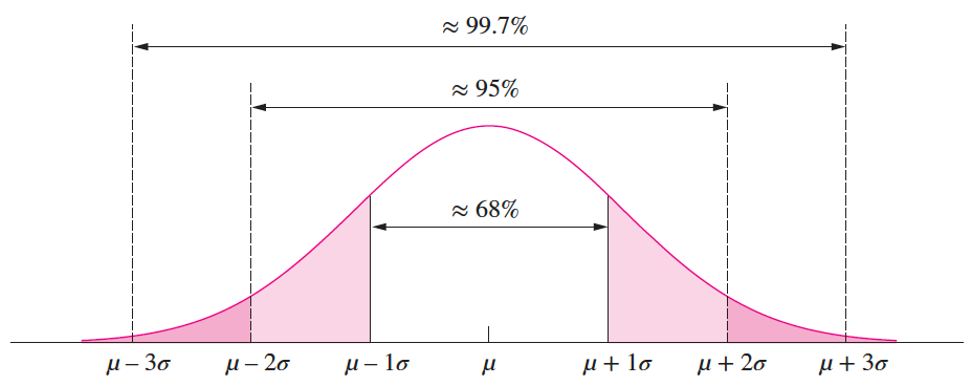
\includegraphics[width=15cm]{Sections/Image/population.png}
\\
\subsubsection*{Standard units}
Standard units tell how many standard deviations an observation is from the population mean.\\
if x is an item sampled from a normal population with mean$\mu$ and variance $\sigma^2$, the standard unit equavalent of x is the z-score of x.
$$z=\frac{x-\mu}{\sigma}$$
The number z is sometimes called the “z-score” of x. The z-score is an item sampled from a normal population with mean 0 and standard deviation of 1. This normal population is called the standard normal population.

\subsection{The Lognormal Distribution}
For data that contain outliers, the normal distribution is generally not appropriate. The \textbf{lognormal distribution}, which is related to the normal distribution, is often a good choice for these data sets.\\
\\
If $X\sim N(\mu, \sigma^2)$, then the random variable $Y=e^X$ has the lognormal distribution with parameters \munsigma.\\
If Y has the lognormal distribution with parameters \munsigma, then the random variable $X=\ln Y$ has the $N(\mu, \sigma^2)$ distribution.\\
\\
The PDF of a lognormal random variable with parameters \munsigma is:
\begin{equation*}
    f(x)=
    \begin{cases}
    \frac{1}{\sigma x \sqrt{2\pi}}e^{-\frac{1}{2\sigma^2}(\ln x-\mu)^2},& , x > 0 \\
    0 &, \mbox{otherwise}
    \end{cases}
\end{equation*}

\subsection{The Exponential Distribution}
The exponential distribution is a continuous distribution that is sometimes used to model the time that elapses before an event occurs. Such a time is often called a waiting time.\\
The probability density of the exponential distribution involves a parameter, which is a positive constant $\lambda$ whose value determines the density function's location and shape.\\
\begin{equation*}
    X\sim e^{\lambda}
\end{equation*}
The PDF of exponential RV:
\begin{equation*}
    f(x)=
    \begin{cases}
    \lambda e^{-\lambda x} &, x>0\\
    0 &, x \leq 0
    \end{cases}
\end{equation*}
The CDF of exponential RV:
\begin{equation*}
    f(x)=
    \begin{cases}
    1-e^{-\lambda x} &, x>0\\
    0 &, x \leq 0
    \end{cases}
\end{equation*}
\begin{align*}
    \mu _x &= \frac{1}{\lambda}\\
    \sigma _x ^2 &= \frac{1}{\lambda^2}
\end{align*}
The exponential distribution is the correct model for waiting times whenever the events follow a Poisson process.\\
If events follow a Poisson process with rate parameter $\lambda$ and if T represents the waiting time from any starting point until the next event, then:
\begin{equation*}
    T\sim e^{\lambda}
\end{equation*}


\subsection{The Uniform Distribution}
The uniform distribution has two parameters, a and b, with a $<$ b. If X is a random variable with the continuous uniform distribution then it is uniformly distributed on the interval (a, b). We write$X\sim U(a,b)$\\
Area of probability is rectangle.\\
$f(x)$ is constant over the possible values of x.\\
The PDF of the uniform distribution:
\begin{equation*}
    f(x)=
    \begin{cases}
    \frac{1}{b-a}, & \mbox{if } c< x < d\\
    0, & \mbox{elsewhere}
    \end{cases}
\end{equation*}
\begin{align*}
    \mu _x &= \frac{a+b}{2}\\
    \sigma _x ^2 &= \frac{(b-a)^2}{12}
\end{align*}
\subsection{The Weibull Distribution}
The Weibull distribution is a continuous random variable that is used in a variety of situations. A common application of the Weibull distribution is to model the lifetimes of components. The Weibull probability density function has two parameters, both positive constants, that determine the location and shape. We denote these parameters $\alpha$ and $\beta$.\\
If $\alpha = 1$, the Weibull distribution is the same as the exponential distribution with $\lambda = \beta$.

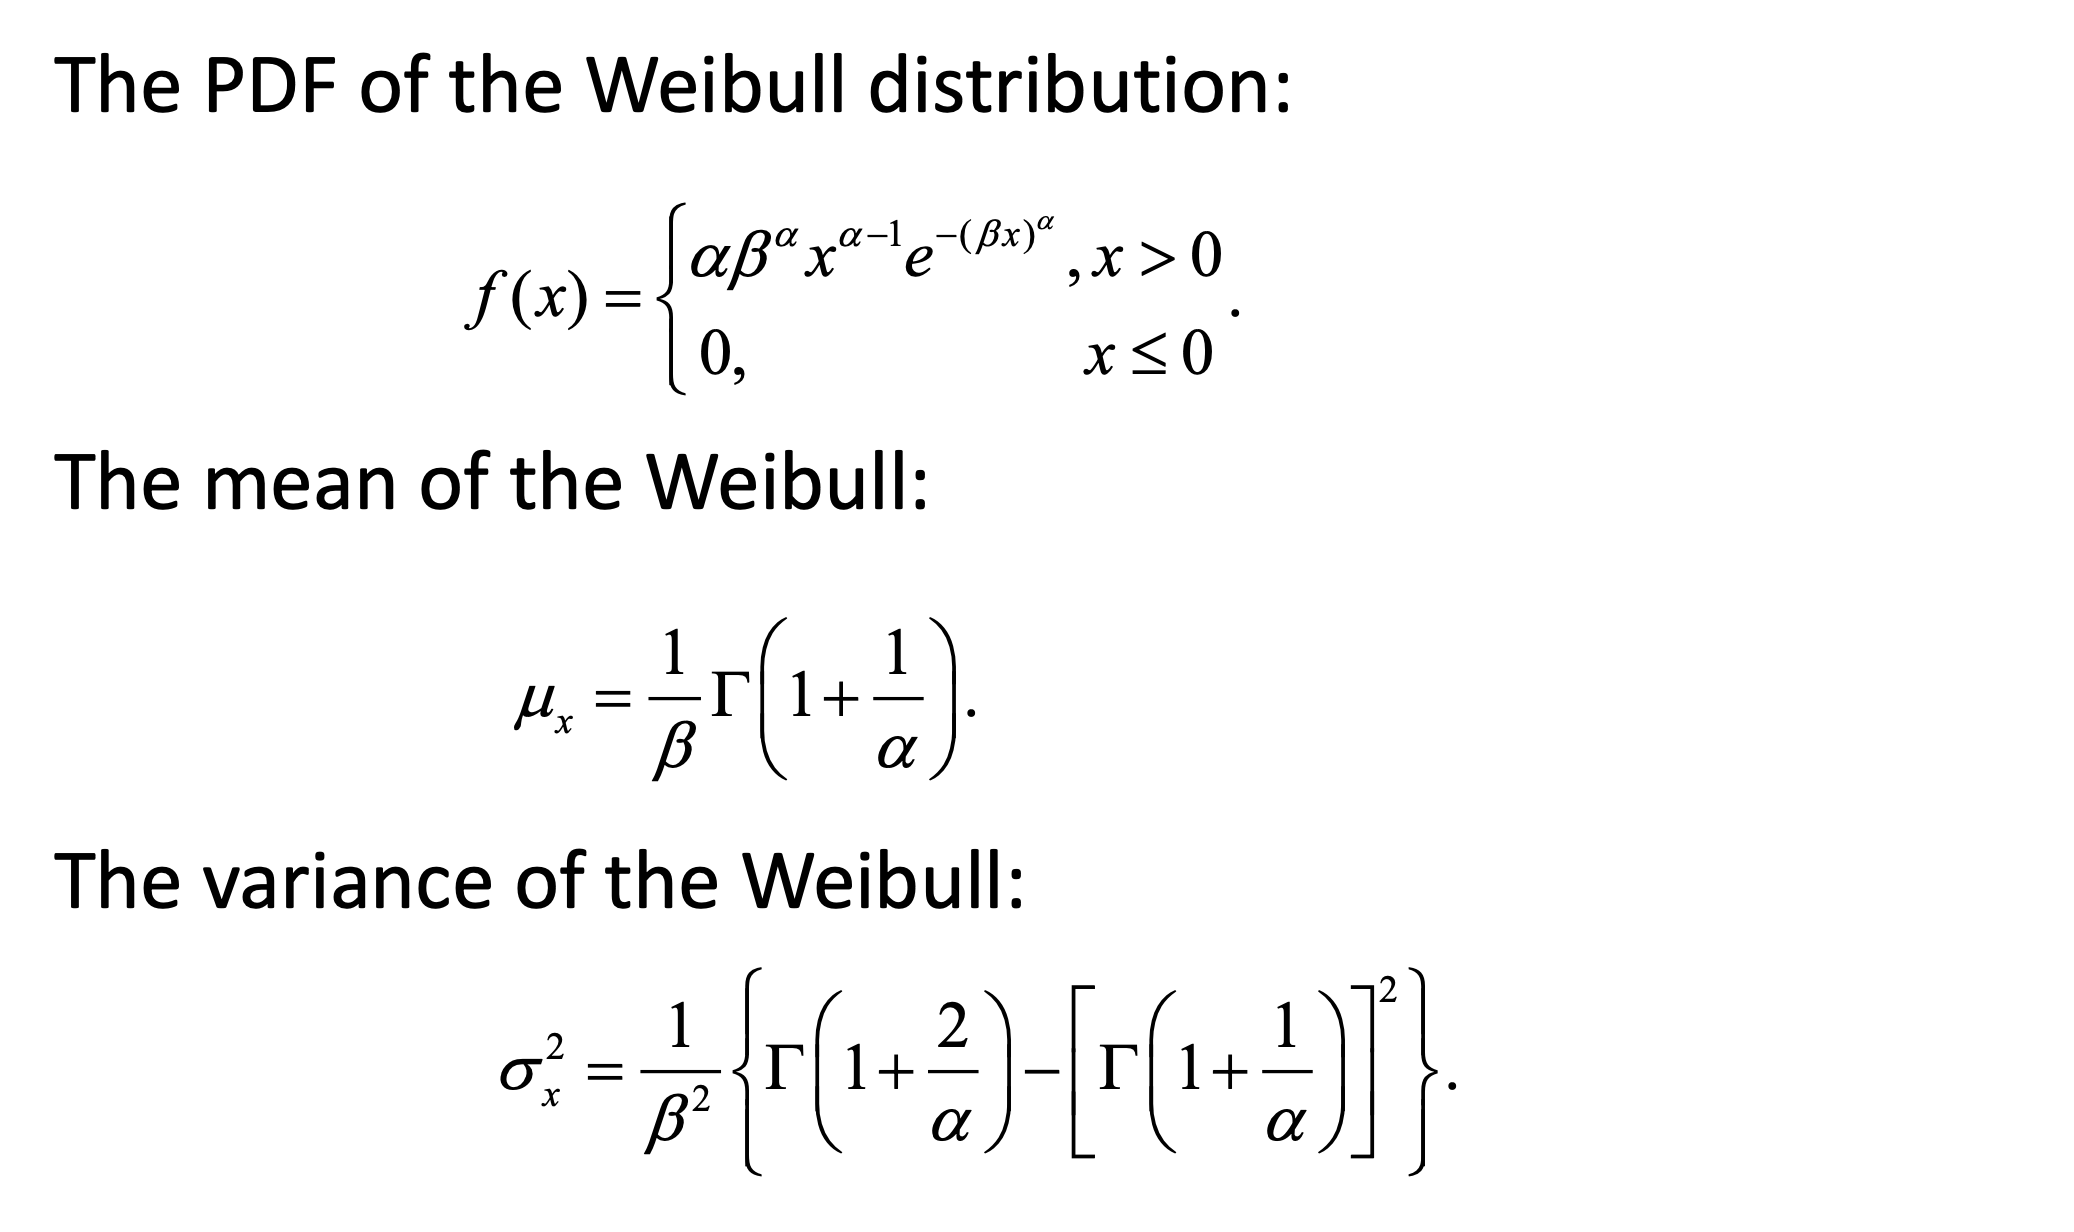
\includegraphics[width = 10cm]{Sections/Image/Weibull.png}\\


\subsection{The Central Limit Theorem}
\textbf{Definition:}\\
If we draw a large enough sample from a population, then the distribution of the sample mean is approximately normal, no matter what population the sample was drawn from.\\

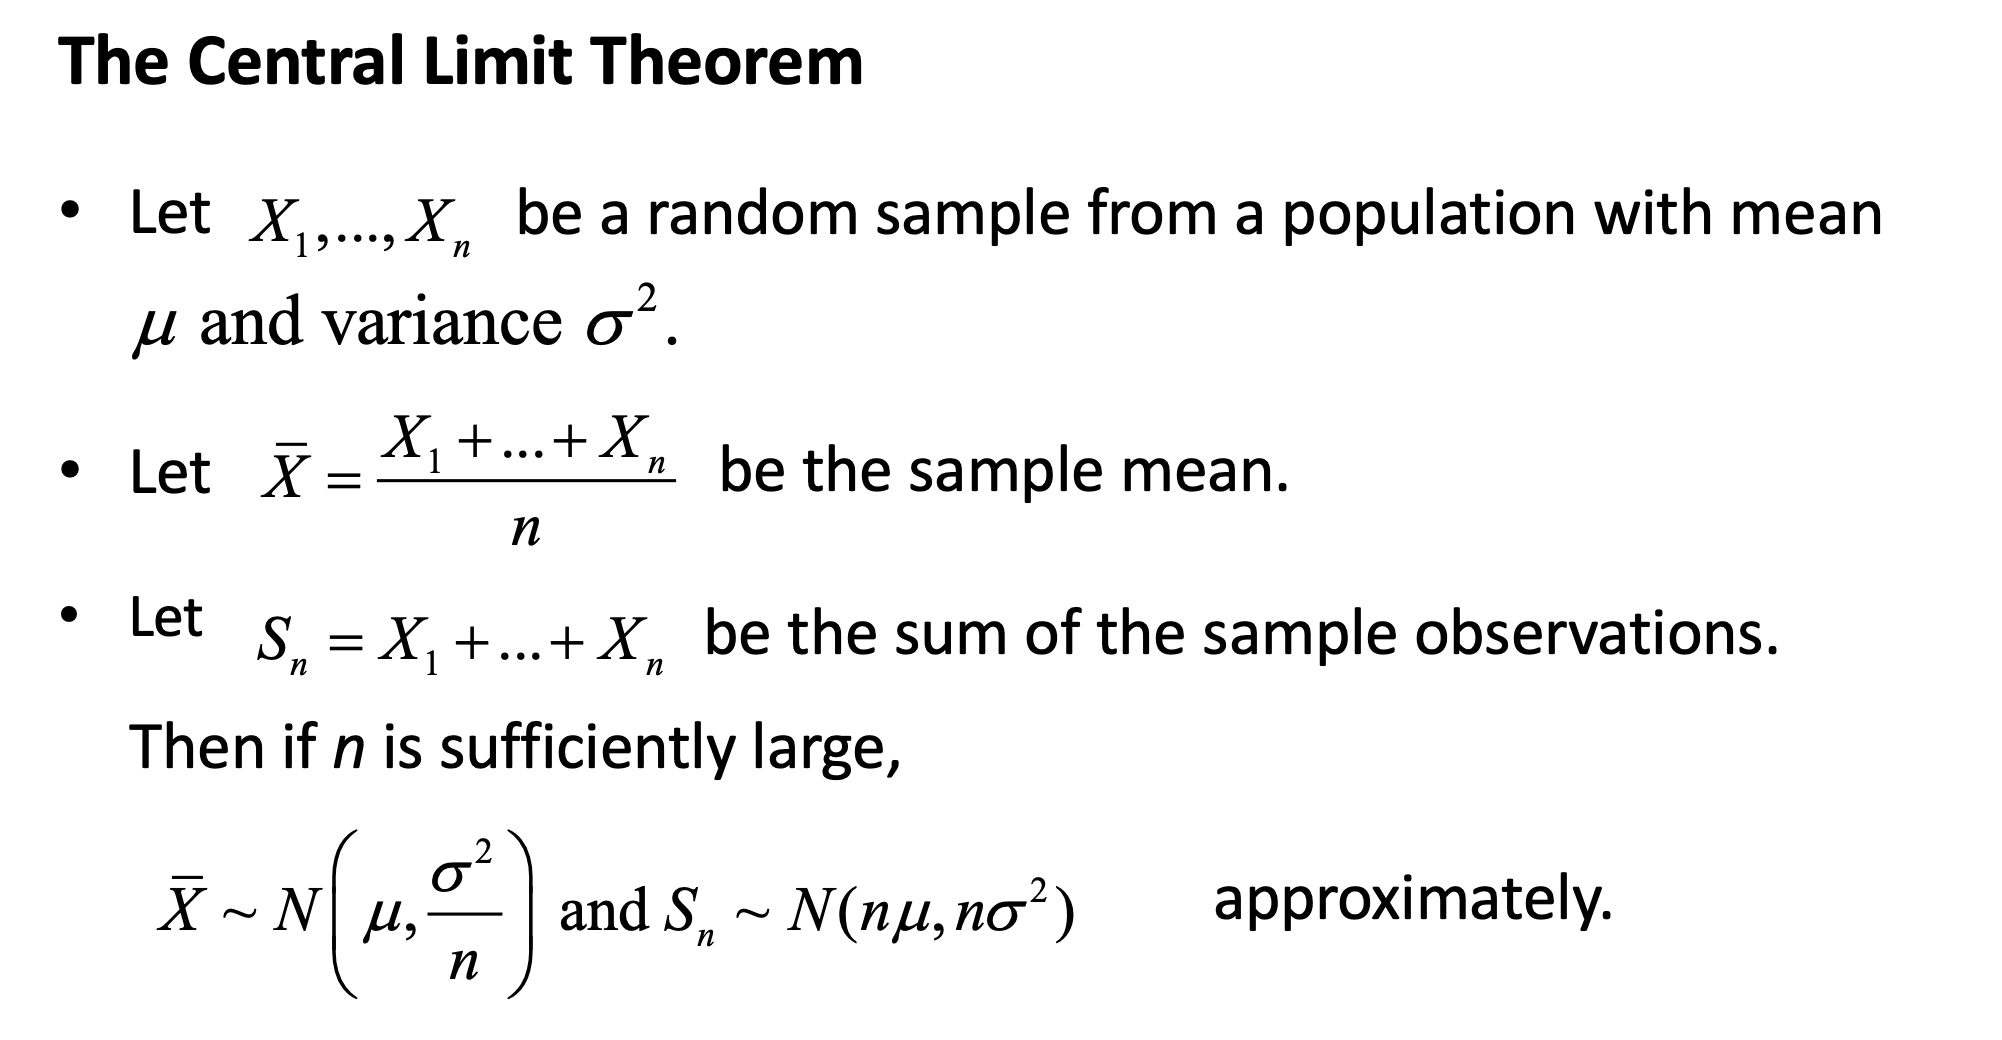
\includegraphics[width = 10cm]{Sections/Image/CLT.png}
\\
The size for CLT:\\
If the sample is drawn from a nearly symmetric distribution, the normal approximation can be good even for a fairly small value of n.\\ 
If the population is heavily skewed, a fairly large n may be necessary. \\
If the sample size is greater than 30, the Central Limit Theorem approximation is good.


\end{document}